Verwandeln Sie die Grammatik
\begin{align*}
K&\to \texttt{(}K\texttt{)}K \\
 &\to \varepsilon
\end{align*}
in Chomsky-Normalform und verwenden Sie die Tabellen-Darstellung
des CYK-Algorithmus, um einen Parse Tree von \texttt{(()(()))}
zu finden.

\thema{CYK-Algorithmus}
\thema{Chomsk-Normalform}

\begin{loesung}
Wir beginnen mit der Umwandlung in CNF.
Im ersten wird sichergestellt, dass die Startvariable auf der rechten
Seite nicht vorkommt:
\begin{align*}
K_0&\to K \\
K  &\to \texttt{(}K\texttt{)}K \\
   &\to \varepsilon
\end{align*}
Die $\varepsilon$-Regel $K\to\varepsilon$ muss entfernt werden:
\begin{align*}
K_0&\to K \mid  \varepsilon\\
K  &\to \texttt{(}K\texttt{)}K \mid  \texttt{()}K \mid  \texttt{(}K\texttt{)} \mid  \texttt{()}\\
\end{align*}
Die einzige Unit-Rule ist $K_0\to K$, sie kann entfernt werden:
\begin{align*}
K_0&\to \texttt{(}K\texttt{)}K \mid  \texttt{()}K \mid  \texttt{(}K\texttt{)} \mid  \texttt{()}
\mid  \varepsilon\\
K  &\to \texttt{(}K\texttt{)}K \mid  \texttt{()}K \mid  \texttt{(}K\texttt{)} \mid  \texttt{()}\\
\end{align*}
Es bleibt nur noch, die Regeln mit mehr als 2 Variablen auf der rechten
Seite zu vereinfachen:
\begin{align*}
K_0
&\to
OA_1
\mid 
OA_2
\mid 
OB
\mid 
OS
\\
K_0&\to
\varepsilon
\\
K
&\to
OA_1
\mid 
OA_2
\mid 
OB
\mid 
OS
\\
A_1&\to KA_2 \\
A_2&\to SK \\
B  &\to KS \\
O&\to \texttt{(} \\
S&\to \texttt{)} \\
\end{align*}
Damit ist die Chomsky-Normalform der Grammatik gefunden.


Um den String \texttt{(()(()))} mit dem CYK-Algorithmus in der Tabellenform
zu parsen beginnen wird damit, die Tabelle aufzustellen, wo wir auch gleich
die Umsetzung in Terminalsymbole in der untersten Zeile eintragen können,
die eindeutig ist. 
\def\h{0.6}
\def\punkt#1#2{
	({(#1)*\h},{(-#2)*\h})
}
\def\tabelle{
	\fill[color=gray!40]
		\punkt{1}{0} -- \punkt{1}{1}
		-- \punkt{2}{1} -- \punkt{2}{2}
		-- \punkt{3}{2} -- \punkt{3}{3}
		-- \punkt{4}{3} -- \punkt{4}{4}
		-- \punkt{5}{4} -- \punkt{5}{5}
		-- \punkt{6}{5} -- \punkt{6}{6}
		-- \punkt{7}{6} -- \punkt{7}{7}
		-- \punkt{8}{7} -- \punkt{8}{0} -- cycle;
	\draw (0,0) rectangle \punkt{8}{8};
	\foreach \x in {1,...,7}{
		\draw \punkt{\x}{0} -- \punkt{\x}{8};
	}
	\foreach \y in {1,...,7}{
		\draw \punkt{0}{\y} -- \punkt{8}{\y};
	}
	\node at \punkt{0.5}{8.5} {\texttt{(}};
	\node at \punkt{1.5}{8.5} {\texttt{(}};
	\node at \punkt{2.5}{8.5} {\texttt{)}};
	\node at \punkt{3.5}{8.5} {\texttt{(}};
	\node at \punkt{4.5}{8.5} {\texttt{(}};
	\node at \punkt{5.5}{8.5} {\texttt{)}};
	\node at \punkt{6.5}{8.5} {\texttt{)}};
	\node at \punkt{7.5}{8.5} {\texttt{)}};
	\node at \punkt{0.5}{7.5} {$O$};
	\node at \punkt{1.5}{7.5} {$O$};
	\node at \punkt{2.5}{7.5} {$S$};
	\node at \punkt{3.5}{7.5} {$O$};
	\node at \punkt{4.5}{7.5} {$O$};
	\node at \punkt{5.5}{7.5} {$S$};
	\node at \punkt{6.5}{7.5} {$S$};
	\node at \punkt{7.5}{7.5} {$S$};
}
\def\zeile#1{
	\fill[color=red!20] \punkt{0}{(#1-1)} rectangle \punkt{#1}{(#1)};
}
\def\zeilezwei{
	\node at \punkt{1.5}{6.5} {$K_{\color{gray}0}$};
	\node at \punkt{4.5}{6.5} {$K_{\color{gray}0}$};
}
\def\zeiledrei{
	\node at \punkt{4.5}{5.5} {$B$};
}
\def\zeilevier{
	\node at \punkt{3.5}{4.5} {$K_{\color{gray}0}$};
}
\def\zeilefuenf{
	\node at \punkt{2.5}{3.5} {$A_2$};
	\node at \punkt{3.5}{3.5} {$B$};
}
\def\zeilesechs{
	\node at \punkt{1.5}{2.5} {$K_{\color{gray}0}$};
}
\def\zeilesieben{
	\node at \punkt{1.5}{1.5} {$B$};
}
\def\zeileacht{
	\node at \punkt{0.5}{0.5} {$K_{\color{gray}0}$};
}
\begin{center}
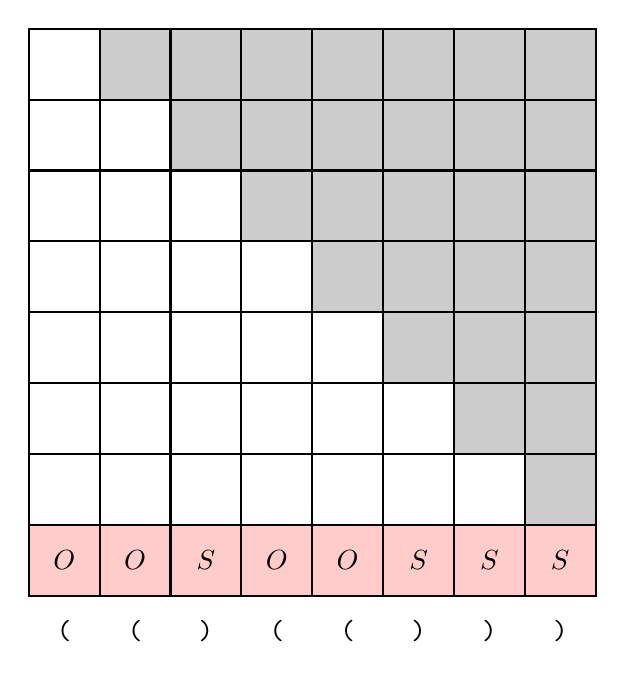
\begin{tikzpicture}[>=latex,thick]
\zeile{8}
\tabelle
\end{tikzpicture}
\end{center}
Damit können jetzt die zweitunterste Zeile gefüllt werden, denn dort
sind nur die Regeln $K\to OS$ anwendbar:
\begin{center}
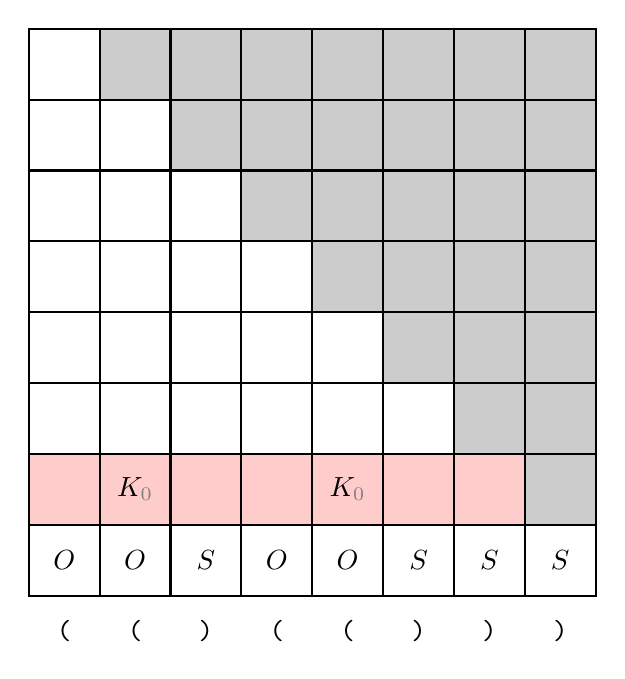
\begin{tikzpicture}[>=latex,thick]
\zeile{7}
\tabelle
\zeilezwei
\end{tikzpicture}
\end{center}
Im Feld $K_{\color{gray}0}$ kann sowohl $K$ und $K_0$ stehen, wir kürzen
dies dadurch ab, dass wir den (optionalen) Index $0$ grau schreiben.
Da aber $K_0$ nicht auf der rechten Seite der Regeln vorkommen kann, 
wird es auch später keine Einträge in Feldern geben, die diese $K_0$
verwenden werden, ausser im Feld in der linken oberen Ecke.

Es wird sich später zeigen, dass das erste $K_{\color{gray}}$ in der
zweituntersten Zeile zwar möglich ist, aber im Parse Tree nicht
gebraucht wird.

Auf diese Weise kann man jetzt die Tabelle zeilenweise füllen:
\begin{center}
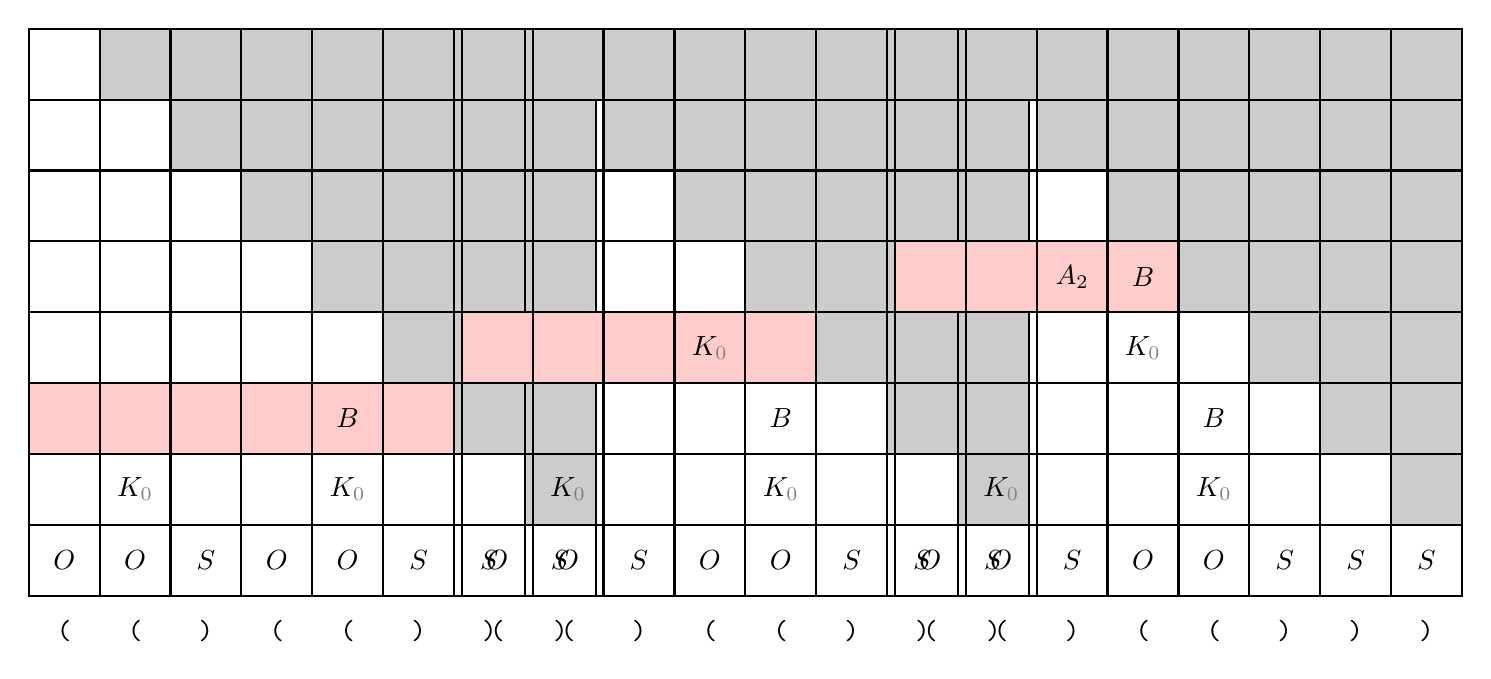
\begin{tikzpicture}[>=latex,thick]
\begin{scope}
	\zeile{6}
	\tabelle
	\zeilezwei
	\zeiledrei
\end{scope}
\begin{scope}[xshift=5.5cm]
	\zeile{5}
	\tabelle
	\zeilezwei
	\zeiledrei
	\zeilevier
\end{scope}
\begin{scope}[xshift=11cm]
	\zeile{4}
	\tabelle
	\zeilezwei
	\zeiledrei
	\zeilevier
	\zeilefuenf
\end{scope}
\end{tikzpicture}
\end{center}
\begin{center}
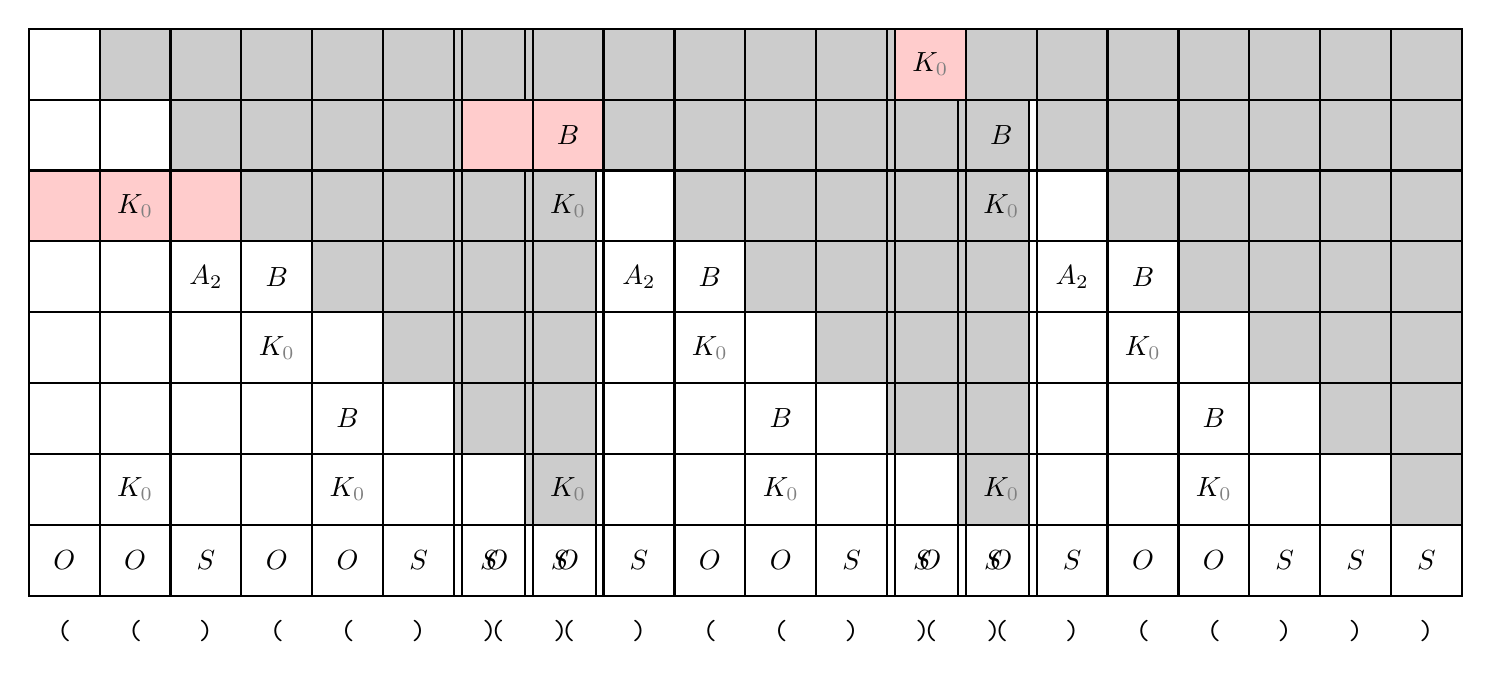
\begin{tikzpicture}[>=latex,thick]
\begin{scope}
	\zeile{3}
	\tabelle
	\zeilezwei
	\zeiledrei
	\zeilevier
	\zeilefuenf
	\zeilesechs
\end{scope}
\begin{scope}[xshift=5.5cm]
	\zeile{2}
	\tabelle
	\zeilezwei
	\zeiledrei
	\zeilevier
	\zeilefuenf
	\zeilesechs
	\zeilesieben
\end{scope}
\begin{scope}[xshift=11cm]
	\zeile{1}
	\tabelle
	\zeilezwei
	\zeiledrei
	\zeilevier
	\zeilefuenf
	\zeilesechs
	\zeilesieben
	\zeileacht
\end{scope}
\end{tikzpicture}
\end{center}
Daraus kann man jetzt den Parse Tree ablesen:
\begin{center}
\def\h{0.9}
\def\pfeil#1#2#3#4{
\draw[->,shorten >= 0.25cm,shorten <= 0.25cm]
	\punkt{#1}{#2} -- \punkt{#3}{#4};
}
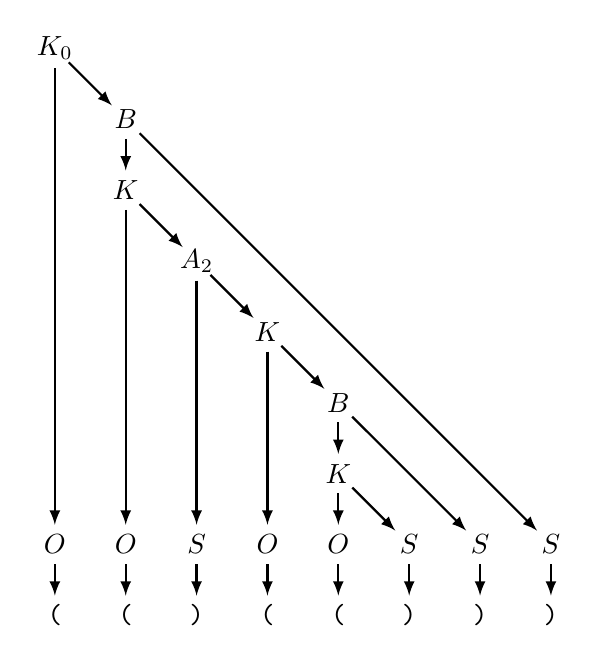
\begin{tikzpicture}[>=latex,thick]
\node at \punkt{0.5}{0.5} {$K_0$};
\pfeil{0.5}{0.5}{0.5}{7.5}
\pfeil{0.5}{0.5}{1.5}{1.5}

\node at \punkt{1.5}{1.5} {$B$};
\pfeil{1.5}{1.5}{1.5}{2.5};
\pfeil{1.5}{1.5}{7.5}{7.5};

\node at \punkt{1.5}{2.5} {$K$};
\pfeil{1.5}{2.5}{1.5}{7.5}
\pfeil{1.5}{2.5}{2.5}{3.5}

\node at \punkt{2.5}{3.5} {$A_2$};
\pfeil{2.5}{3.5}{2.5}{7.5}
\pfeil{2.5}{3.5}{3.5}{4.5}

\node at \punkt{3.5}{4.5} {$K$};
\pfeil{3.5}{4.5}{3.5}{7.5}
\pfeil{3.5}{4.5}{4.5}{5.5}

\node at \punkt{4.5}{5.5} {$B$};
\pfeil{4.5}{5.5}{4.5}{6.5}
\pfeil{4.5}{5.5}{6.5}{7.5}

\node at \punkt{4.5}{6.5} {$K$};
\pfeil{4.5}{6.5}{4.5}{7.5}
\pfeil{4.5}{6.5}{5.5}{7.5}

\pfeil{0.5}{7.5}{0.5}{8.5}
\pfeil{1.5}{7.5}{1.5}{8.5}
\pfeil{2.5}{7.5}{2.5}{8.5}
\pfeil{3.5}{7.5}{3.5}{8.5}
\pfeil{4.5}{7.5}{4.5}{8.5}
\pfeil{5.5}{7.5}{5.5}{8.5}
\pfeil{6.5}{7.5}{6.5}{8.5}
\pfeil{7.5}{7.5}{7.5}{8.5}

\node at \punkt{0.5}{7.5}{$O$};
\node at \punkt{1.5}{7.5}{$O$};
\node at \punkt{2.5}{7.5}{$S$};
\node at \punkt{3.5}{7.5}{$O$};
\node at \punkt{4.5}{7.5}{$O$};
\node at \punkt{5.5}{7.5}{$S$};
\node at \punkt{6.5}{7.5}{$S$};
\node at \punkt{7.5}{7.5}{$S$};

\node at \punkt{0.5}{8.5} {\texttt{(}};
\node at \punkt{1.5}{8.5} {\texttt{(}};
\node at \punkt{2.5}{8.5} {\texttt{)}};
\node at \punkt{3.5}{8.5} {\texttt{(}};
\node at \punkt{4.5}{8.5} {\texttt{(}};
\node at \punkt{5.5}{8.5} {\texttt{)}};
\node at \punkt{6.5}{8.5} {\texttt{)}};
\node at \punkt{7.5}{8.5} {\texttt{)}};
\end{tikzpicture}
\end{center}
\end{loesung}
